\chapter{第一次作业题目}
\section{题目描述}
已知转移矩阵为:

\begin{equation}
    L = 
    \begin{bmatrix}
        0.6 & 0.1 & 0.3\\
        0.1 & 0.9 & 0\\
        0.3 & 0 & 0.7\\
    \end{bmatrix}
\end{equation}

初始状态为$x_0 = [2,1,1] ^ T$

求$x_k = L^k x_0$ 和 稳定态 $\displaystyle \lim_{k \to \infty} x_k$

\section{求解过程}

\subsection{Step1.先求出$L$的特征向量}

求解矩阵$L$的特征方程得
\begin{equation}
    \begin{split}  
   |\lambda E - A | &= 
   \begin{vmatrix}
    \lambda - 0.6 & -0.1 & -0.3\\
    -0.1 & \lambda - 0.9 & 0\\
    -0.3 & 0 & \lambda -0.7\\
   \end{vmatrix}
   \\
   &=(\lambda -0.6)(\lambda - 0.9)(\lambda-0.7)-0.3·0.3·(\lambda - 0.9) + 0.1·0.1·(\lambda - 0.7)\\
   &= \lambda ^ 3 - 2.2 \lambda ^ 2 + 1.49 \lambda - 0.29
\end{split}
\end{equation}

运用sympy求特征值和特征向量得

特征值:
\begin{equation}
\lambda_1 = 1, \lambda_2 =\frac{6-\sqrt[]{7}}{10}, \lambda_3 = \frac{6 + \sqrt[]{7}}{10}
\end{equation}

从而得到特征向量为

\begin{equation}
    \displaystyle
\xi_1 = \begin{bmatrix}
    1\\
    1\\
    1\\
\end{bmatrix}
,
\xi_2 =\begin{bmatrix}
    \dfrac{-(7+3\sqrt[]{7})}{(2\sqrt[]{7} + 7)}\\
    \vspace{1.5ex}
    \dfrac{3}{6+3\sqrt[]{7}}\\
    \vspace{1.5ex}
    1\\
\end{bmatrix}
,
\xi_3 =\begin{bmatrix}
    \dfrac{-(-7+3\sqrt[]{7})}{(2\sqrt[]{7} - 7)}\\
    \vspace{1.5ex}
    \dfrac{3}{6-3\sqrt[]{7}}\\
    \vspace{1.5ex}
    1\\
\end{bmatrix}
\end{equation}

\subsection{Step2.将$L$相似对角化并求解}
因此可以将$L$相似对角化成 $L=PDP^{-1}$的形式,其中
\begin{equation}
P = \begin{bmatrix}
    1  & \dfrac{-\sqrt[]{7} - 1}{3} & \dfrac{\sqrt[]{7} - 1}{3} \\
    \vspace{1.5ex}
    1  & \dfrac{\sqrt[]{7} -2}{3}& \dfrac{-\sqrt[]{7} - 2}{3}\\
    \vspace{1.5ex}
    1  & 1                                          & 1\\
\end{bmatrix},
D = \begin{bmatrix}
    10 & 0 & 0\\
    \vspace{1.5ex}
    0  & 6-\sqrt[]{7} & 0\\
    \vspace{1.5ex}
    0 & 0 & 6 + \sqrt[]{7}\\
\end{bmatrix}
\end{equation}

所以有

\begin{equation}
    \begin{split}
        x_k &= L^k x_0\\
        &= (\frac{1}{10})^k · L'^{k} x_0\\
        &= (\frac{1}{10})^k · P\begin{bmatrix}
            \lambda_1^k & 0 & 0\\
            0 & \lambda_2^k & 0\\
            0 & 0 & \lambda_3^k\\
        \end{bmatrix} P^{-1} · \begin{bmatrix}
            2\\1\\1
        \end{bmatrix}\\
        % &= \begin{bmatrix}
        %     \frac{4*10^k}{3} - \frac{3(\sqrt[]{7} + 1)(6-\sqrt[]{7})^k}{28-2\sqrt[]{7}} 
        %     - \frac{(\sqrt[]{7} + 1)(3\sqrt[]{7} - 6)(6-\sqrt[]{7})^k}{3*(28-2\sqrt[]{7})} 
        %     +  \frac{2(\sqrt[]{7} + 1)(3\sqrt[]{7} + 3)(6-\sqrt[]{7})^k}{3*(28-2\sqrt[]{7})} 
        %     +  (\sqrt[]{7}/3 - 1/3)(-2\sqrt[]{7}/21 - 1/6)(6+\sqrt[]{7})^k 
        %     + (\sqrt[]{7}/3 - 1/3)(-\sqrt[]{7}/42 + 1/3)(6+\sqrt[]{7})^k
        % \end{bmatrix}
    \end{split}
\end{equation}

利用sympy库求得最终解析解为:
\begin{python}
Matrix([[3*(3/5 - sqrt(7)/10)**k*(-sqrt(7)/3 - 1/3)/(28/3 - 2*sqrt(7)/3) - 
(-6 + 3*sqrt(7))*(3/5 - sqrt(7)/10)**k*(-sqrt(7)/3 - 1/3)/(-28 + 2*sqrt(7)) +
 2*(3/5 - sqrt(7)/10)**k*(3 + 3*sqrt(7))*(-sqrt(7)/3 - 1/3)/(-28 + 2*sqrt(7)) + 
 (-1/3 + sqrt(7)/3)*(-2*sqrt(7)/21 - 1/6)*(sqrt(7)/10 + 3/5)**k + 
 (-1/3 + sqrt(7)/3)*(1/3 - sqrt(7)/42)*(sqrt(7)/10 + 3/5)**k + 
 2*(-1/3 + sqrt(7)/3)*(-1/6 + 5*sqrt(7)/42)*(sqrt(7)/10 + 3/5)**k + 4/3],
 
  [2*(-2/3 + sqrt(7)/3)*(3/5 - sqrt(7)/10)**k*(3 + 3*sqrt(7))/(-28 + 2*sqrt(7)) -
   (-6 + 3*sqrt(7))*(-2/3 + sqrt(7)/3)*(3/5 - sqrt(7)/10)**k/(-28 + 2*sqrt(7)) + 
   3*(-2/3 + sqrt(7)/3)*(3/5 - sqrt(7)/10)**k/(28/3 - 2*sqrt(7)/3) + 
   2*(-1/6 + 5*sqrt(7)/42)*(-sqrt(7)/3 - 2/3)*(sqrt(7)/10 + 3/5)**k + 
   (1/3 - sqrt(7)/42)*(-sqrt(7)/3 - 2/3)*(sqrt(7)/10 + 3/5)**k + 
   (-sqrt(7)/3 - 2/3)*(-2*sqrt(7)/21 - 1/6)*(sqrt(7)/10 + 3/5)**k + 4/3], 
   
   [2*(3/5 - sqrt(7)/10)**k*(3 + 3*sqrt(7))/(-28 + 2*sqrt(7)) - 
   (-6 + 3*sqrt(7))*(3/5 - sqrt(7)/10)**k/(-28 + 2*sqrt(7)) +
    3*(3/5 - sqrt(7)/10)**k/(28/3 - 2*sqrt(7)/3) + 
    (-2*sqrt(7)/21 - 1/6)*(sqrt(7)/10 + 3/5)**k + (1/3 - sqrt(7)/42)*(sqrt(7)/10 + 3/5)**k + 
    2*(-1/6 + 5*sqrt(7)/42)*(sqrt(7)/10 + 3/5)**k + 4/3]])
\end{python}

\subsection{Step3.用numpy重写以上过程,求出数值解}

得到
\begin{python}
    特征值:[0.33542487 1.         0.86457513]
特征向量:[[ 0.76505532 -0.57735027  0.28523152]
 [-0.13550992 -0.57735027 -0.8051731 ]
 [-0.6295454  -0.57735027  0.51994159]]
相似对角化后P:
Matrix([[-0.765055323929465, -0.285231516480645, 0.577350269189626], [0.135509922732534, 0.805173104063772, 0.577350269189626], [0.629545401196931, -0.519941587583127, 0.577350269189626]])
相似对角化后D:
Matrix([[0.335424868893541, 0, 0], [0, 0.864575131106459, 0], [0, 0, 1.00000000000000]])
最终解为:
Matrix([[0.585309648672818*0.335424868893541**k + 0.0813570179938488*0.864575131106459**k + 1.33333333333333*1.0**k], 
[-0.103672587831795*0.335424868893541**k - 0.229660745501538*0.864575131106459**k + 1.33333333333333*1.0**k],
 [-0.481637060841023*0.335424868893541**k + 0.14830372750769*0.864575131106459**k + 1.33333333333333*1.0**k]])

\end{python}

\subsection{Step4.求稳定值}

根据矩阵$L$的特征值可知,$\lambda_1 > \lambda_2, \lambda_1 > \lambda_3$。

设矩阵$L$属于特征值$\lambda_i(i=1,2,3)$的特征向量为$\alpha_i$。

根据Step1中算出的特征向量可知,属于特征值$\lambda_1=1$的特征向量为$\alpha_1 = [1,1,1]^T$。

记矩阵$P=[\alpha_1, \alpha_2, \alpha_3]$, $A = diag(\lambda_1, \lambda_2, \lambda_3)$,则有
\begin{equation}
    \begin{split}
    L &=PAP^{-1}
    \\
    L^k &= PA^kP^{-1} 
    \end{split}
\end{equation}

于是有

\begin{equation}
 x_k = L^kx_0 = PA^kP^{-1}x_0 = \lambda_1^kP\begin{bmatrix}
    1 & 0 & 0\\
    0 & (\dfrac{\lambda_2}{\lambda_1})^k& 0\\
    0 & 0 & (\dfrac{\lambda_3}{\lambda_1})^k\\ 
 \end{bmatrix}P^{-1}x_0
\end{equation}

可得

\begin{equation}
    \dfrac{1}{\lambda_1 ^ k}x_k  = P\begin{bmatrix}
       1 & 0 & 0\\
       0 & (\dfrac{\lambda_2}{\lambda_1})^k & 0\\
       0 & 0 &( \dfrac{\lambda_3}{\lambda_1})^k\ 
    \end{bmatrix}P^{-1}x_0
   \end{equation}
   
由于$|\dfrac{\lambda_2}{\lambda_1}| < 1, |\dfrac{\lambda_3}{\lambda_1}| < 1 $

设向量$P^{-1}x_0$的第一个元素为$c$,于是有

\begin{equation}
    \lim_{k\rightarrow\infty}\dfrac{1}{\lambda_1 ^ k}x_k  = P\begin{bmatrix}
       1 & 0 & 0\\
       0 & 0& 0\\
       0 & 0 & 0\\ 
    \end{bmatrix}P^{-1}x_0
    = [\alpha_1, \alpha_2, \alpha_3][c,0,0]^{T} = c\alpha_1
   \end{equation}

当k充分大时,有


\begin{equation}
    x_k = c\lambda_1^k\alpha_1 = c(1)^k\begin{bmatrix}
        1\\
        1\\
        1\\
    \end{bmatrix}
\end{equation}

由sympy解得,$c = \frac{4}{3}$,即
$\lim_{k\rightarrow\infty}x_k = 
\begin{bmatrix}
    \frac{4}{3}\\
    \frac{4}{3}\\
    \frac{4}{3}\\
\end{bmatrix}$

\subsection{Step5.利用numpy直接求解的数值}
% Please add the following required packages to your document preamble:
% \usepackage[table,xcdraw]{xcolor}
% If you use beamer only pass "xcolor=table" option, i.e. \documentclass[xcolor=table]{beamer}
利用numpy库求出$x_k$的前20个数值解,作表\ref{tab:x}

\begin{table}[H]

    \centering
    \caption[]{前20个解}
    \label{tab:x}
    \begin{tabular}{llll}
    \hline
                                       & \multicolumn{3}{c}{ $x_k$}                                                                                                         \\
    \multicolumn{1}{c}{ k} & \multicolumn{1}{c}{ $x_k[1]$} & \multicolumn{1}{c}{ $x_k[2]$} & \multicolumn{1}{c}{ $x_k[3]$} \\ \hline
     1                     & 1.6                                      & 1.1                                         & 1.2999999999999998                       \\
     2                     & 1.46                                     & 1.1500000000000001                          & 1.3899999999999997                       \\
     3                     & 1.408                                    & 1.181                                       & 1.4109999999999998                       \\
     4                     & 1.3861999999999999                       & 1.2037000000000002                          & 1.4100999999999997                       \\
     5                     & 1.37512                                  & 1.22195                                     & 1.4029299999999996                       \\
     6                     & 1.3681459999999999                       & 1.2372670000000001                          & 1.3945869999999996                       \\
     7                     & 1.3629904                                & 1.2503549                                   & 1.3866546999999996                       \\
     8                     & 1.3588261399999997                       & 1.26161845                                  & 1.3795554099999996                       \\
     9                     & 1.3553241519999997                       & 1.2713392190000001                          & 1.3733366289999995                       \\
     10                    & 1.3523294017999996                       & 1.2797377123                                & 1.3679328858999995                       \\
     11                    & 1.3497512780799996                       & 1.28699688125                               & 1.3632518406699994                       \\
     12                    & 1.3475260071739994                       & 1.293272320933                              & 1.3592016718929993                       \\
     13                    & 1.3456033379655994                       & 1.2986976895571                             & 1.3556989724772992                       \\
     14                    & 1.3439414634782594                       & 1.30338825439795                            & 1.3526702821237893                       \\
     15                    & 1.3425047881638874                       & 1.307443575305981                           & 1.3500516365301303                       \\
     16                    & 1.3412627213879695                       & 1.3109496965917717                          & 1.3477875820202574                       \\
     17                    & 1.3401888770980361                       & 1.3139809990713915                          & 1.345830123830571                        \\
     18                    & 1.3392604633151322                       & 1.316601786874056                           & 1.3441377498108105                       \\
     19                    & 1.338457781619728                        & 1.3188676545181637                          & 1.342674563862107                        \\
     20                    & 1.3377638035822852                       & 1.3208266672283202                          & 1.3414095291893933                       \\ \hline
    \end{tabular}
\end{table}

求出前100个数值解并作图\ref{fig:img},可以看出k足够大时,稳定在$\lim_{k\rightarrow\infty}x_k = 
\begin{bmatrix}
    \frac{4}{3}\\
    \frac{4}{3}\\
    \frac{4}{3}\\
\end{bmatrix}$

\begin{figure}[htbp]
    \begin{center}
        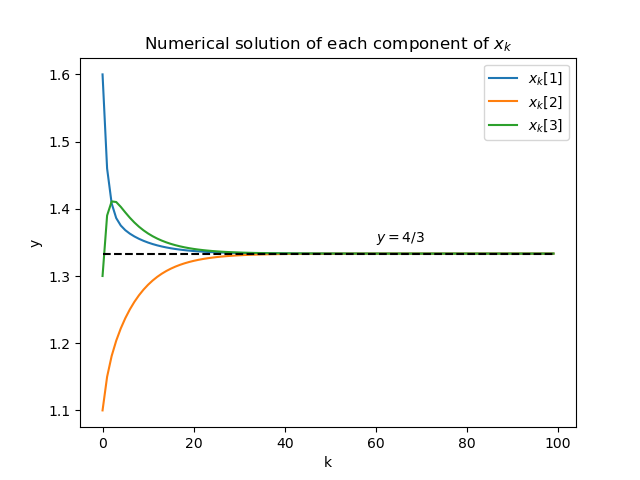
\includegraphics[width=0.7\textwidth]{img.png}
    \end{center}
   \caption[]{前100项$x_k$各分量值}
    \label{fig:img}
\end{figure}